\subsection*{2.4  Cách tiếp cận dự kiến}
\myparagraph{Bản mẫu}
\begin{figure}[H]
    \centering
    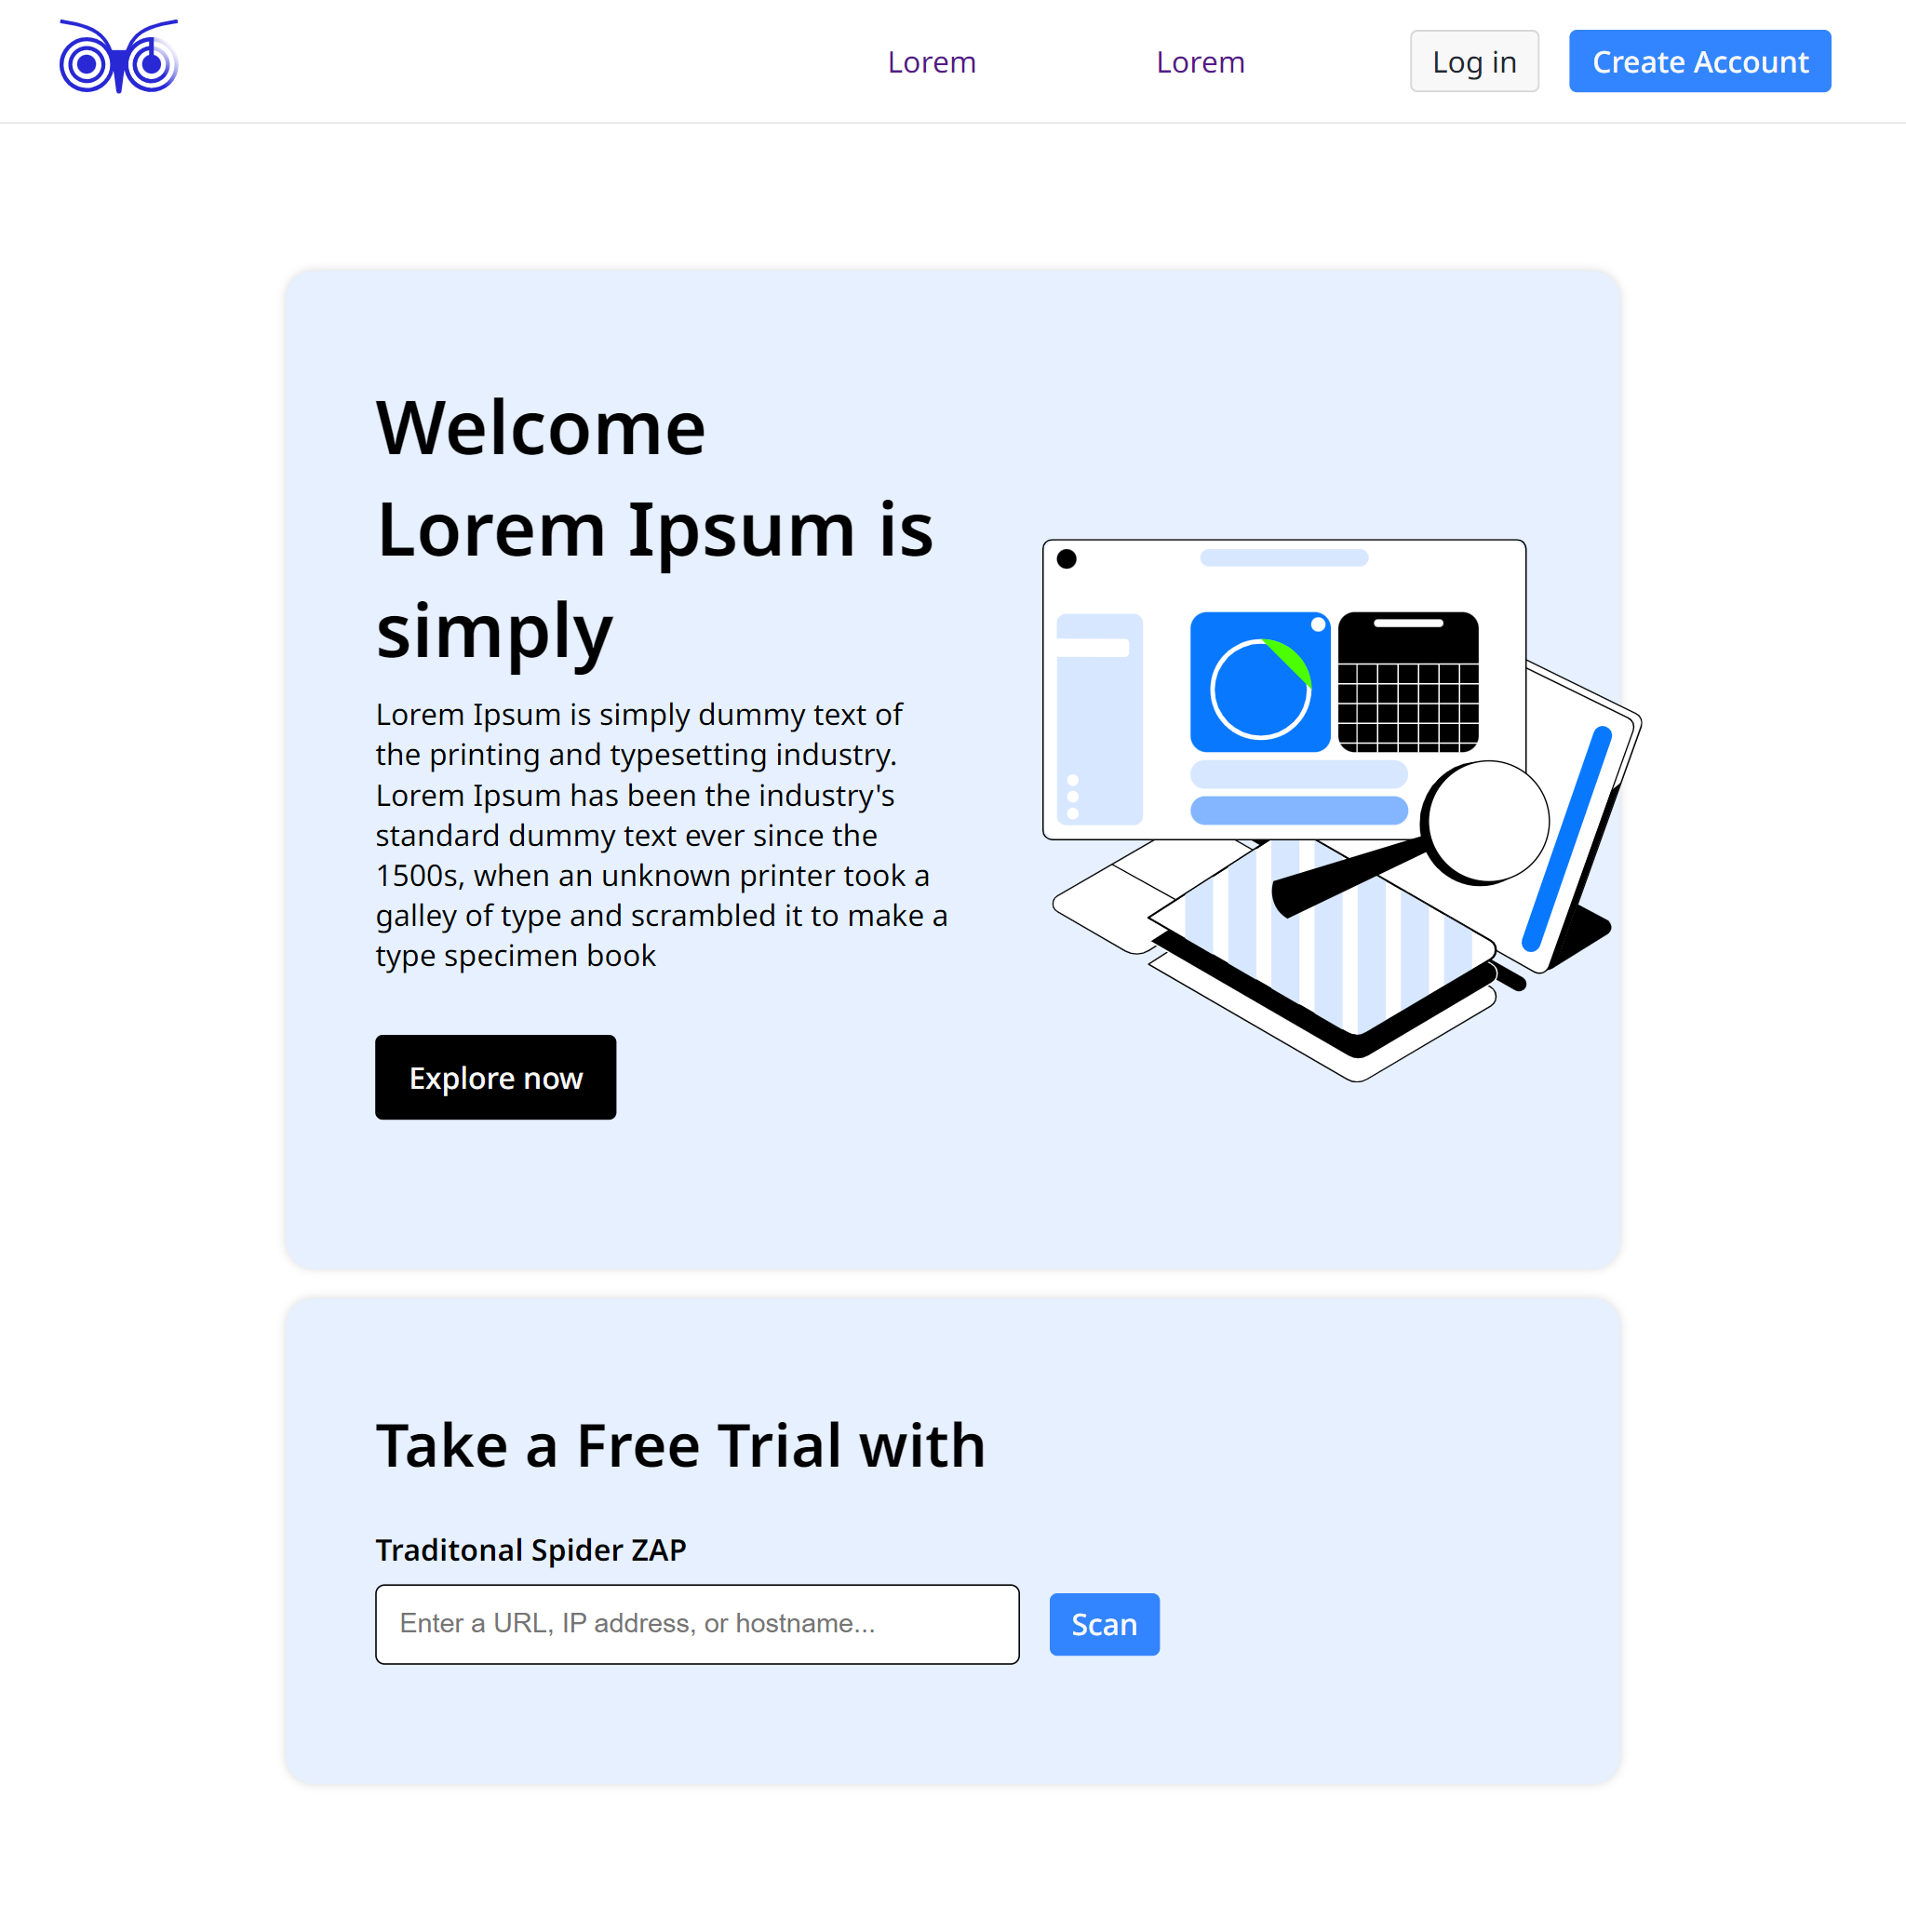
\includegraphics[width=\textwidth]{images/prototype/prototype_22112022/home.png}
    \caption{Màn hình trang chủ của ứng dụng}
\end{figure}

\begin{figure}[H]
    \centering
    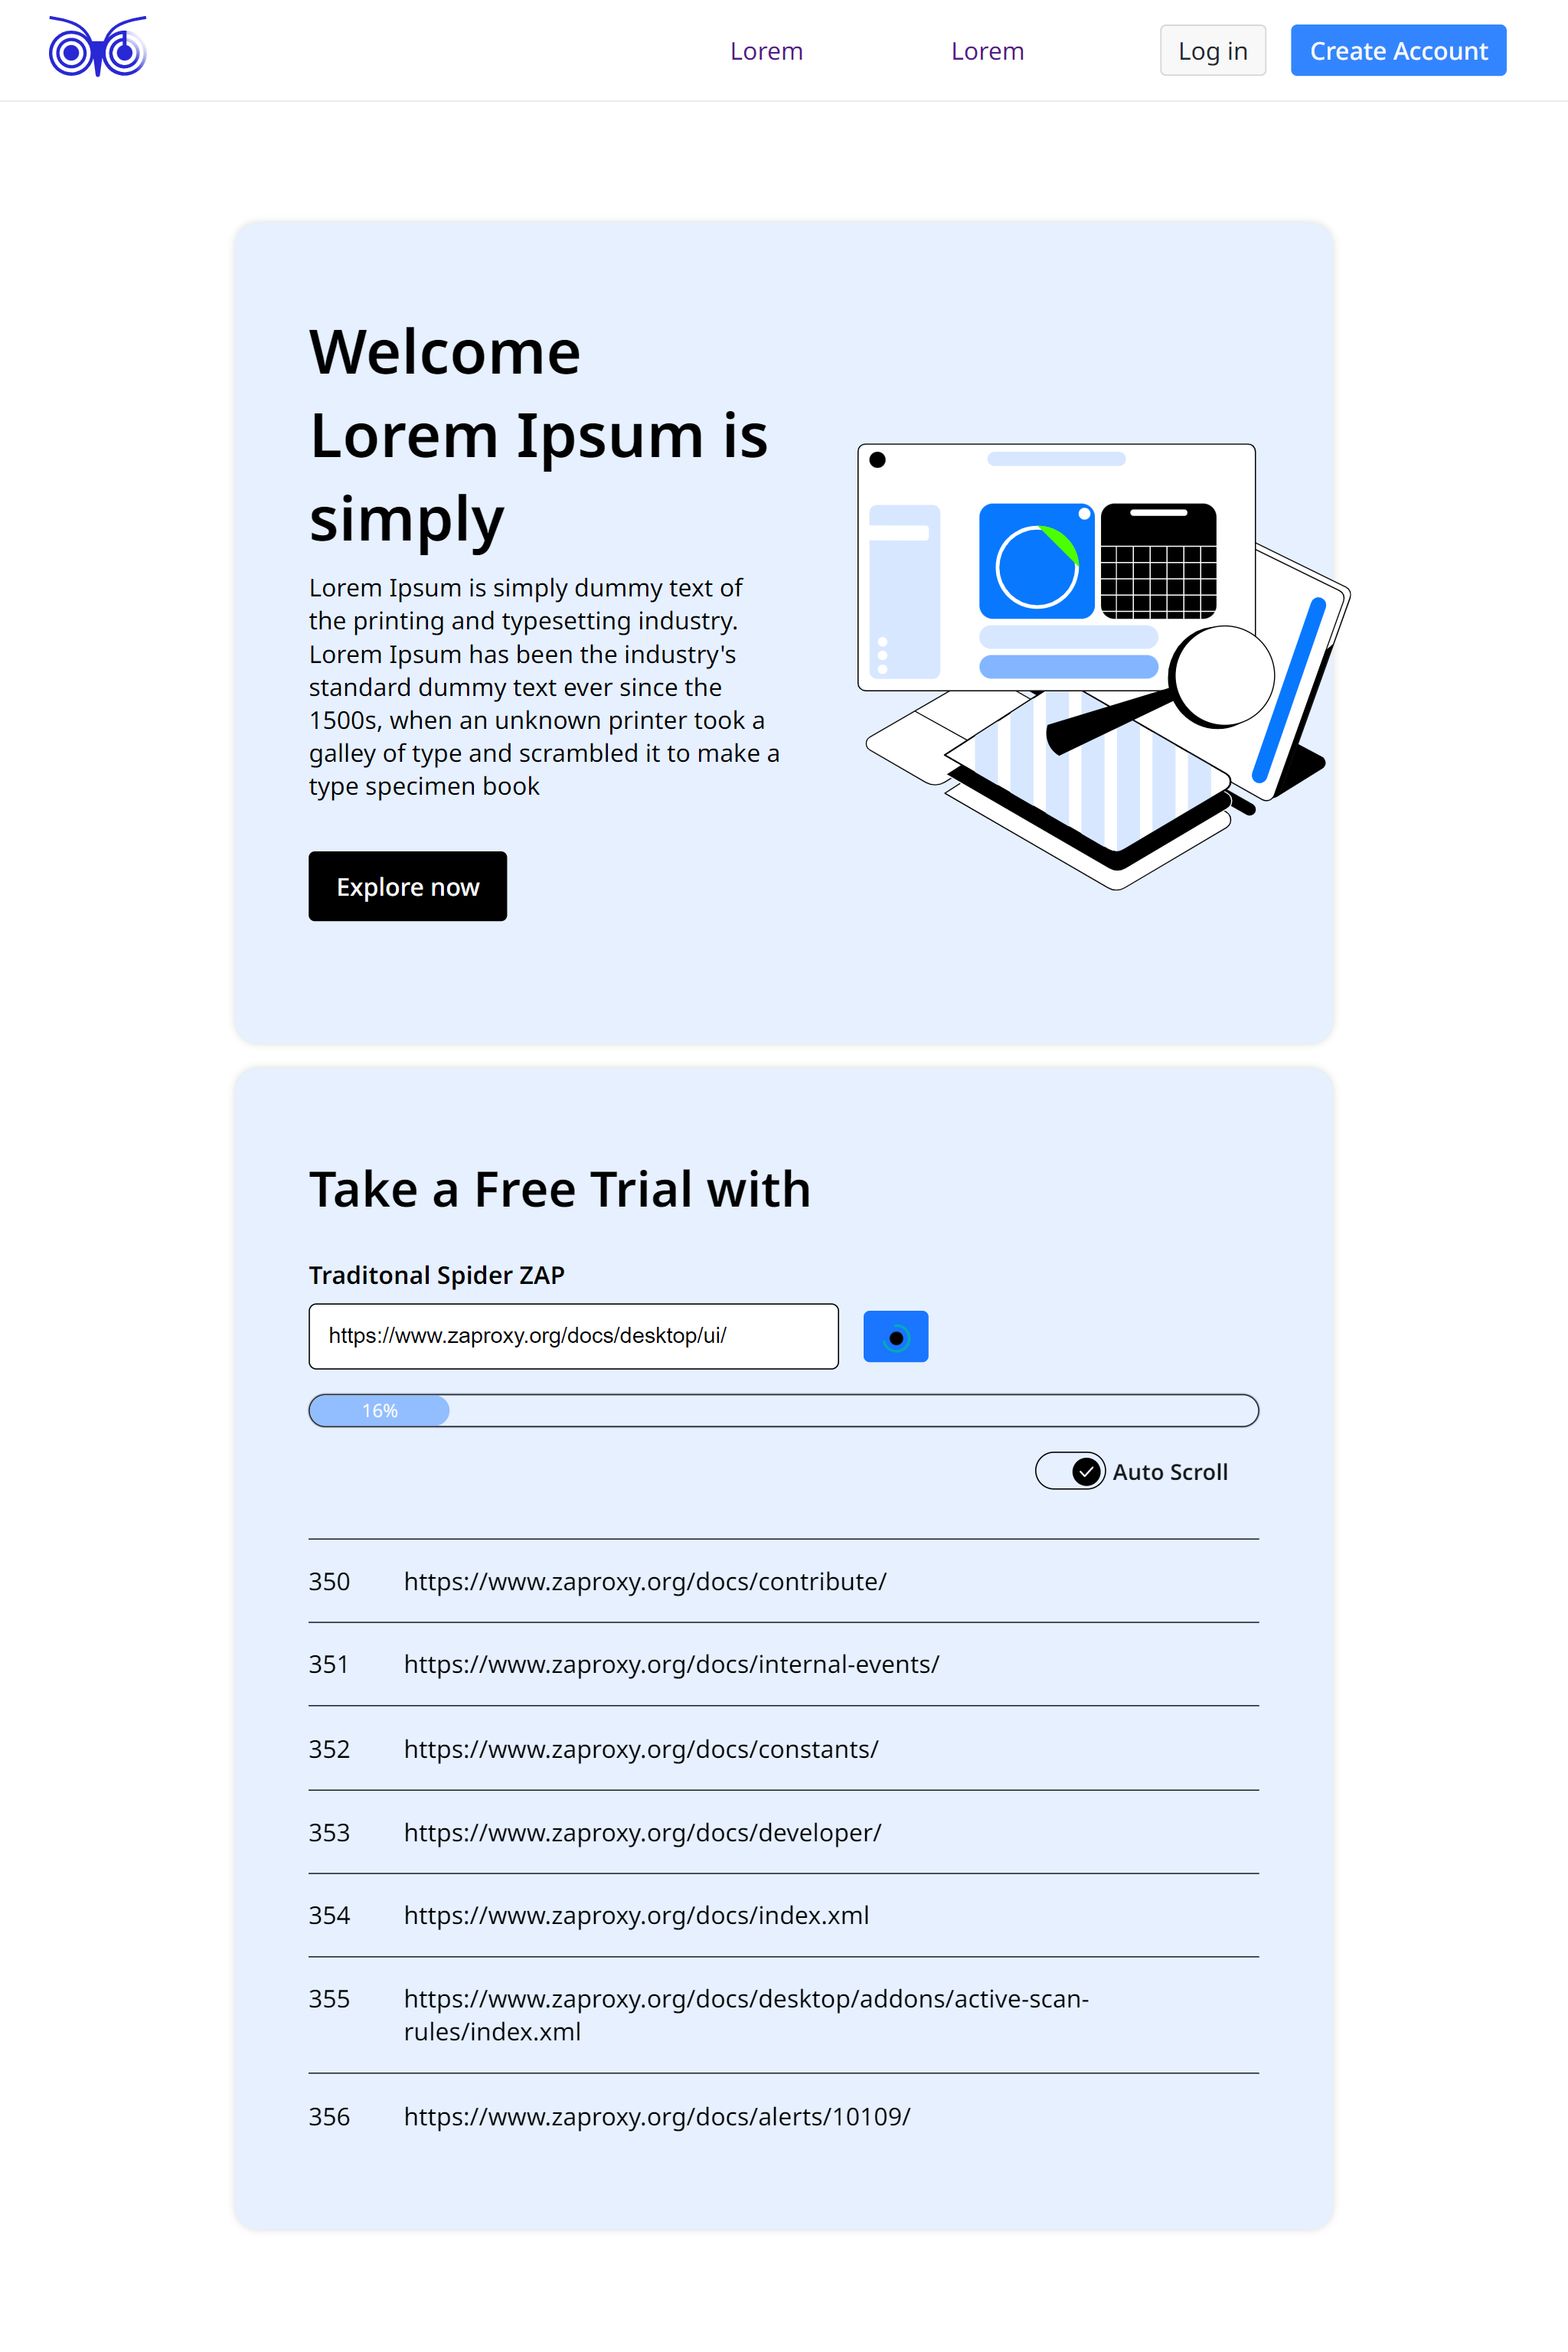
\includegraphics[width=\textwidth]{images/prototype/prototype_22112022/home_scanning.png}
    \caption{Màn hình trang chủ của ứng dụng đang thực hiện chức năng quét thử với ZAP Spider}
\end{figure}

\begin{figure}[H]
    \centering
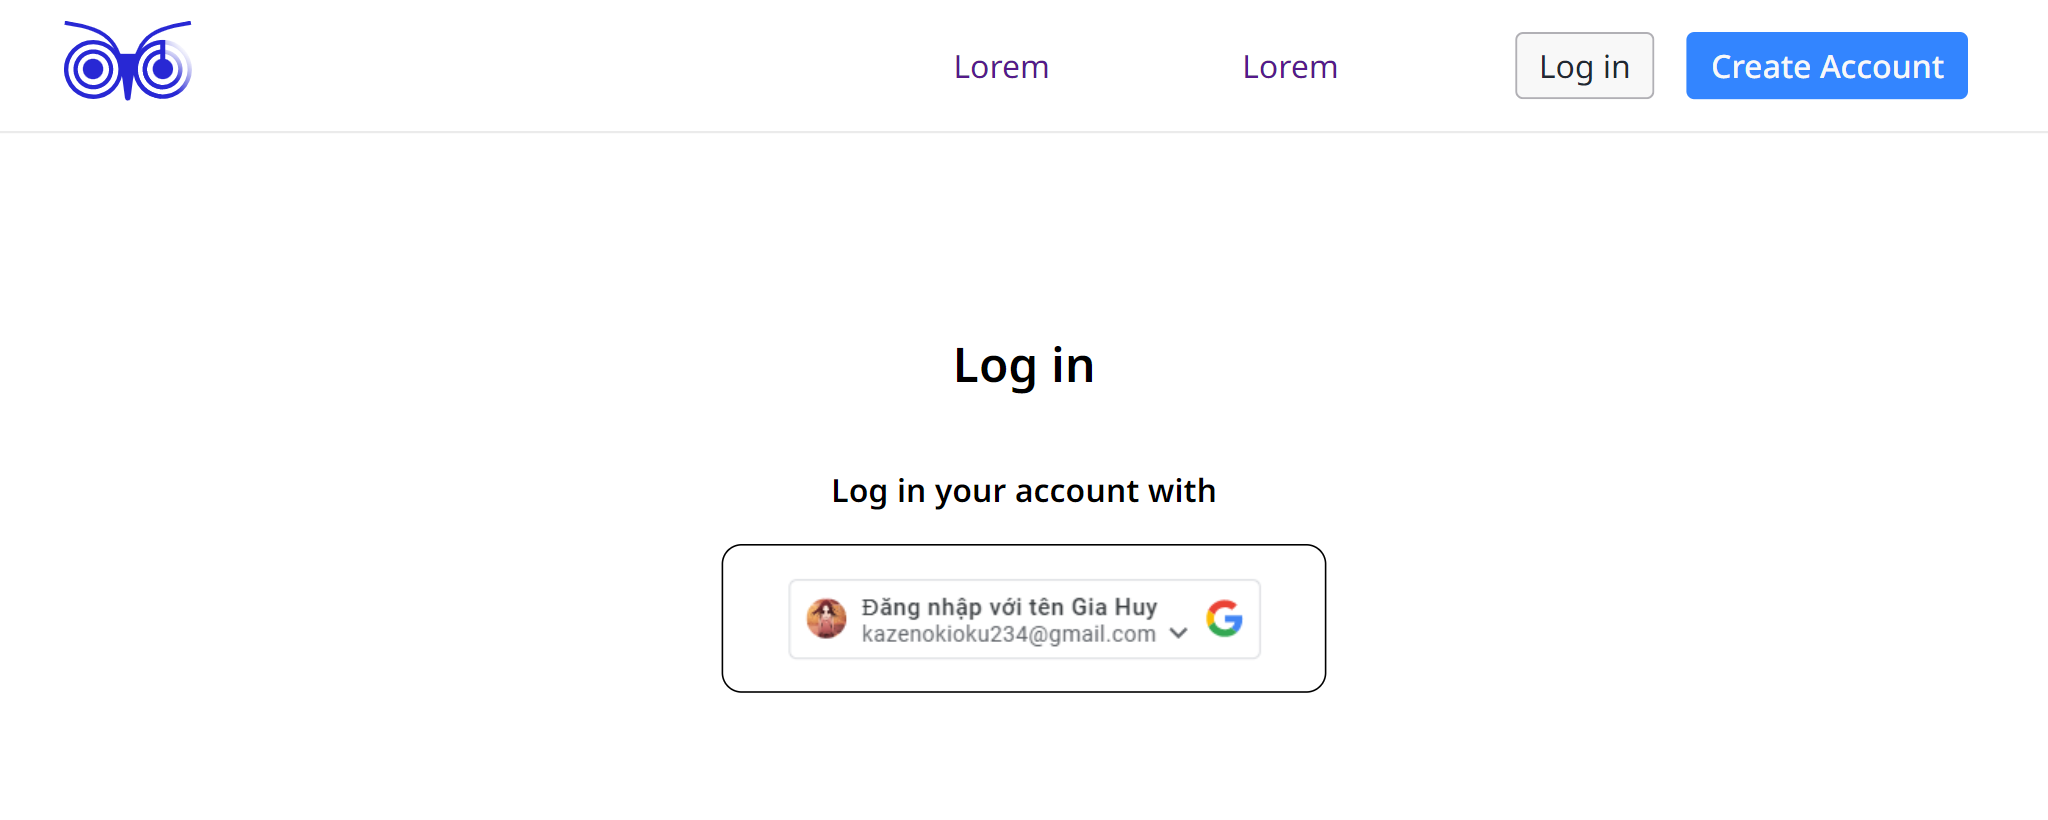
\includegraphics[width=\textwidth]{images/prototype/prototype_22112022/login.png}
    \caption{Màn hình trang đăng nhập và đăng ký của ứng dụng}
\end{figure}

\begin{figure}[H]
    \centering
    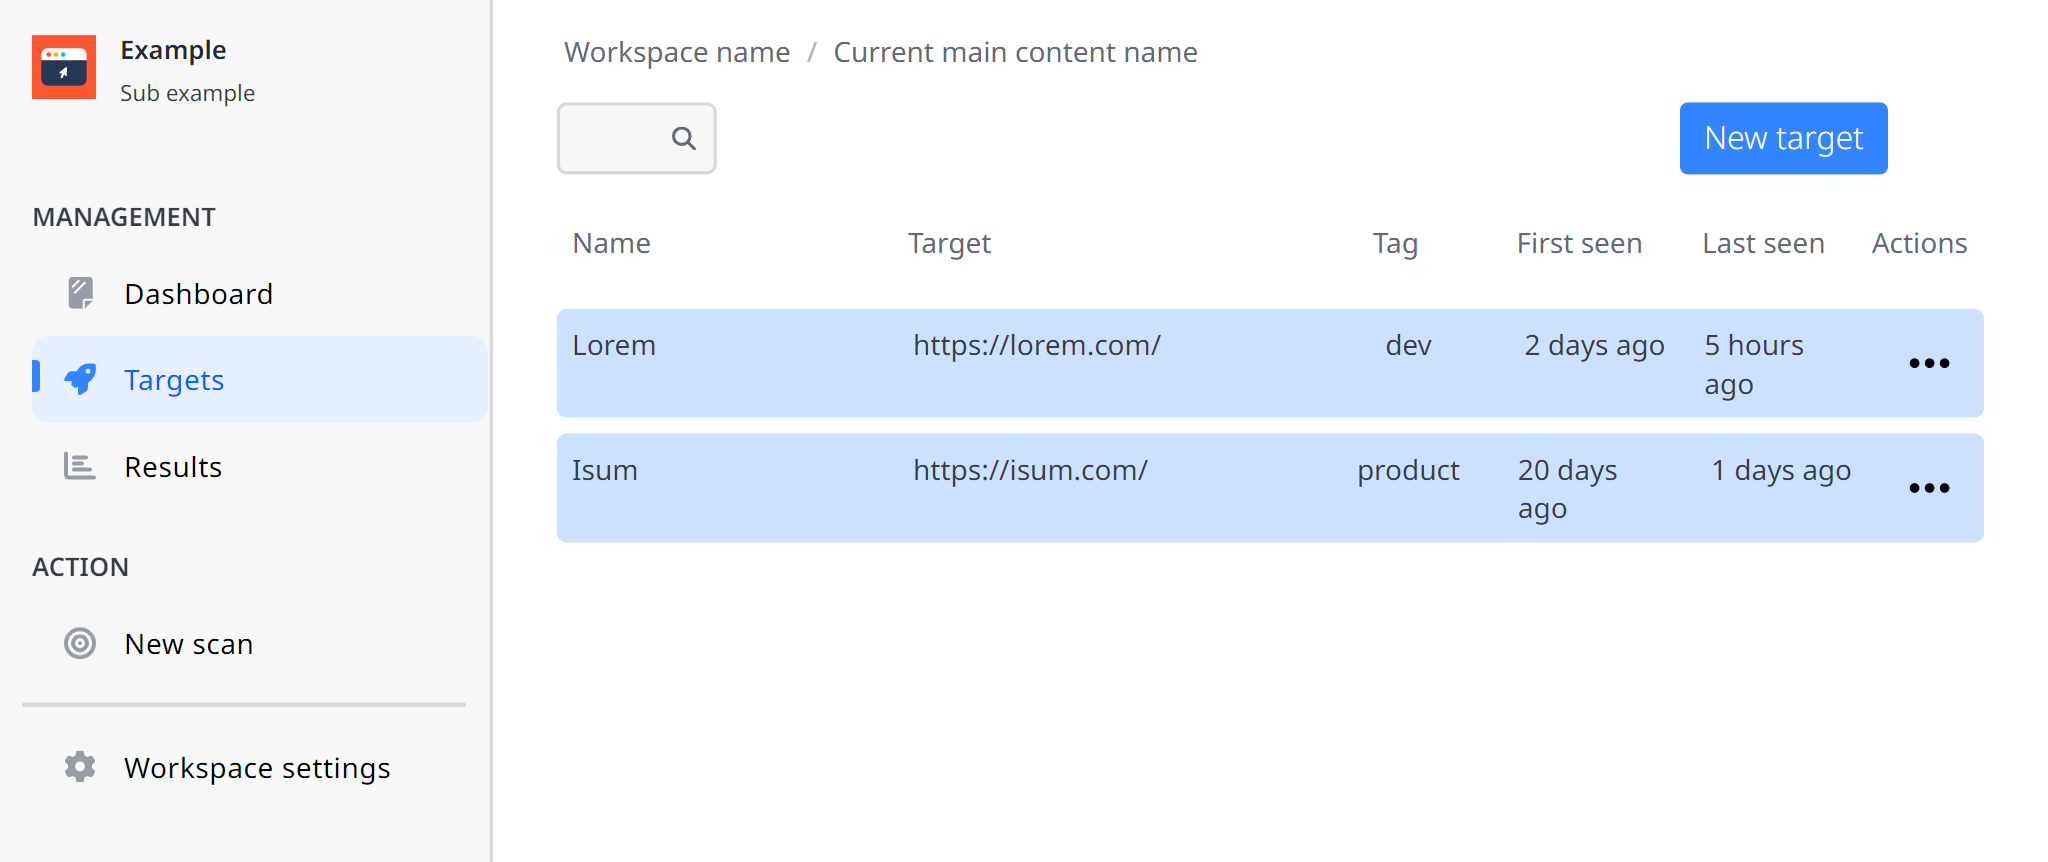
\includegraphics[width=\textwidth]{images/prototype/prototype_22112022/dashboard_target.png}
    \caption{Màn hình trang quản lý mục tiêu của ứng dụng }
\end{figure}

\begin{figure}[H]
    \centering
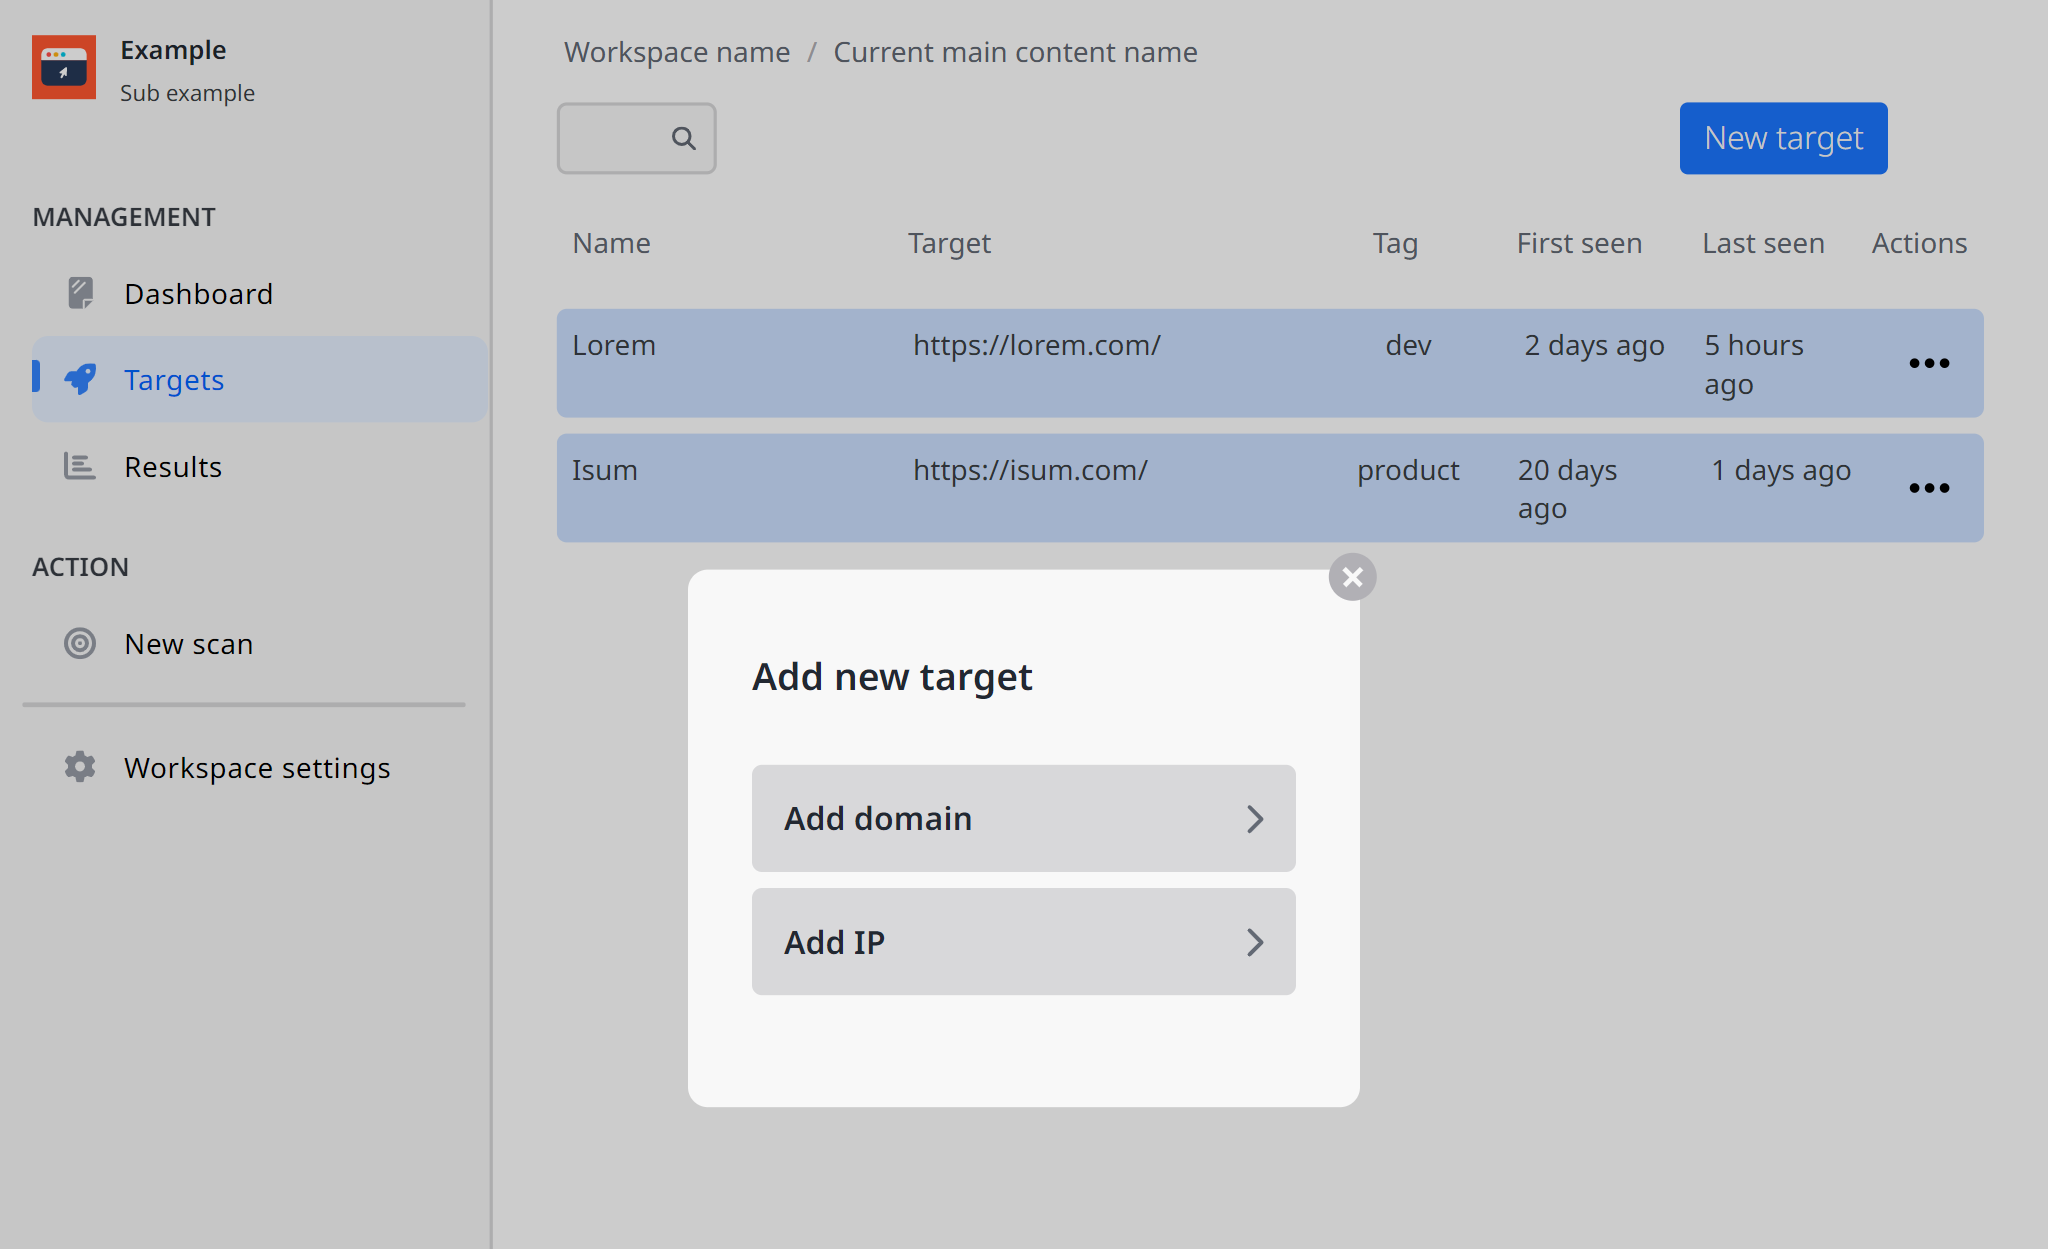
\includegraphics[width=\textwidth]{images/prototype/prototype_22112022/dashboard_target_add target.png}
    \caption{Màn hình trang thêm mới mục tiêu của ứng dụng 1}
\end{figure}

\begin{figure}[H]
    \centering
    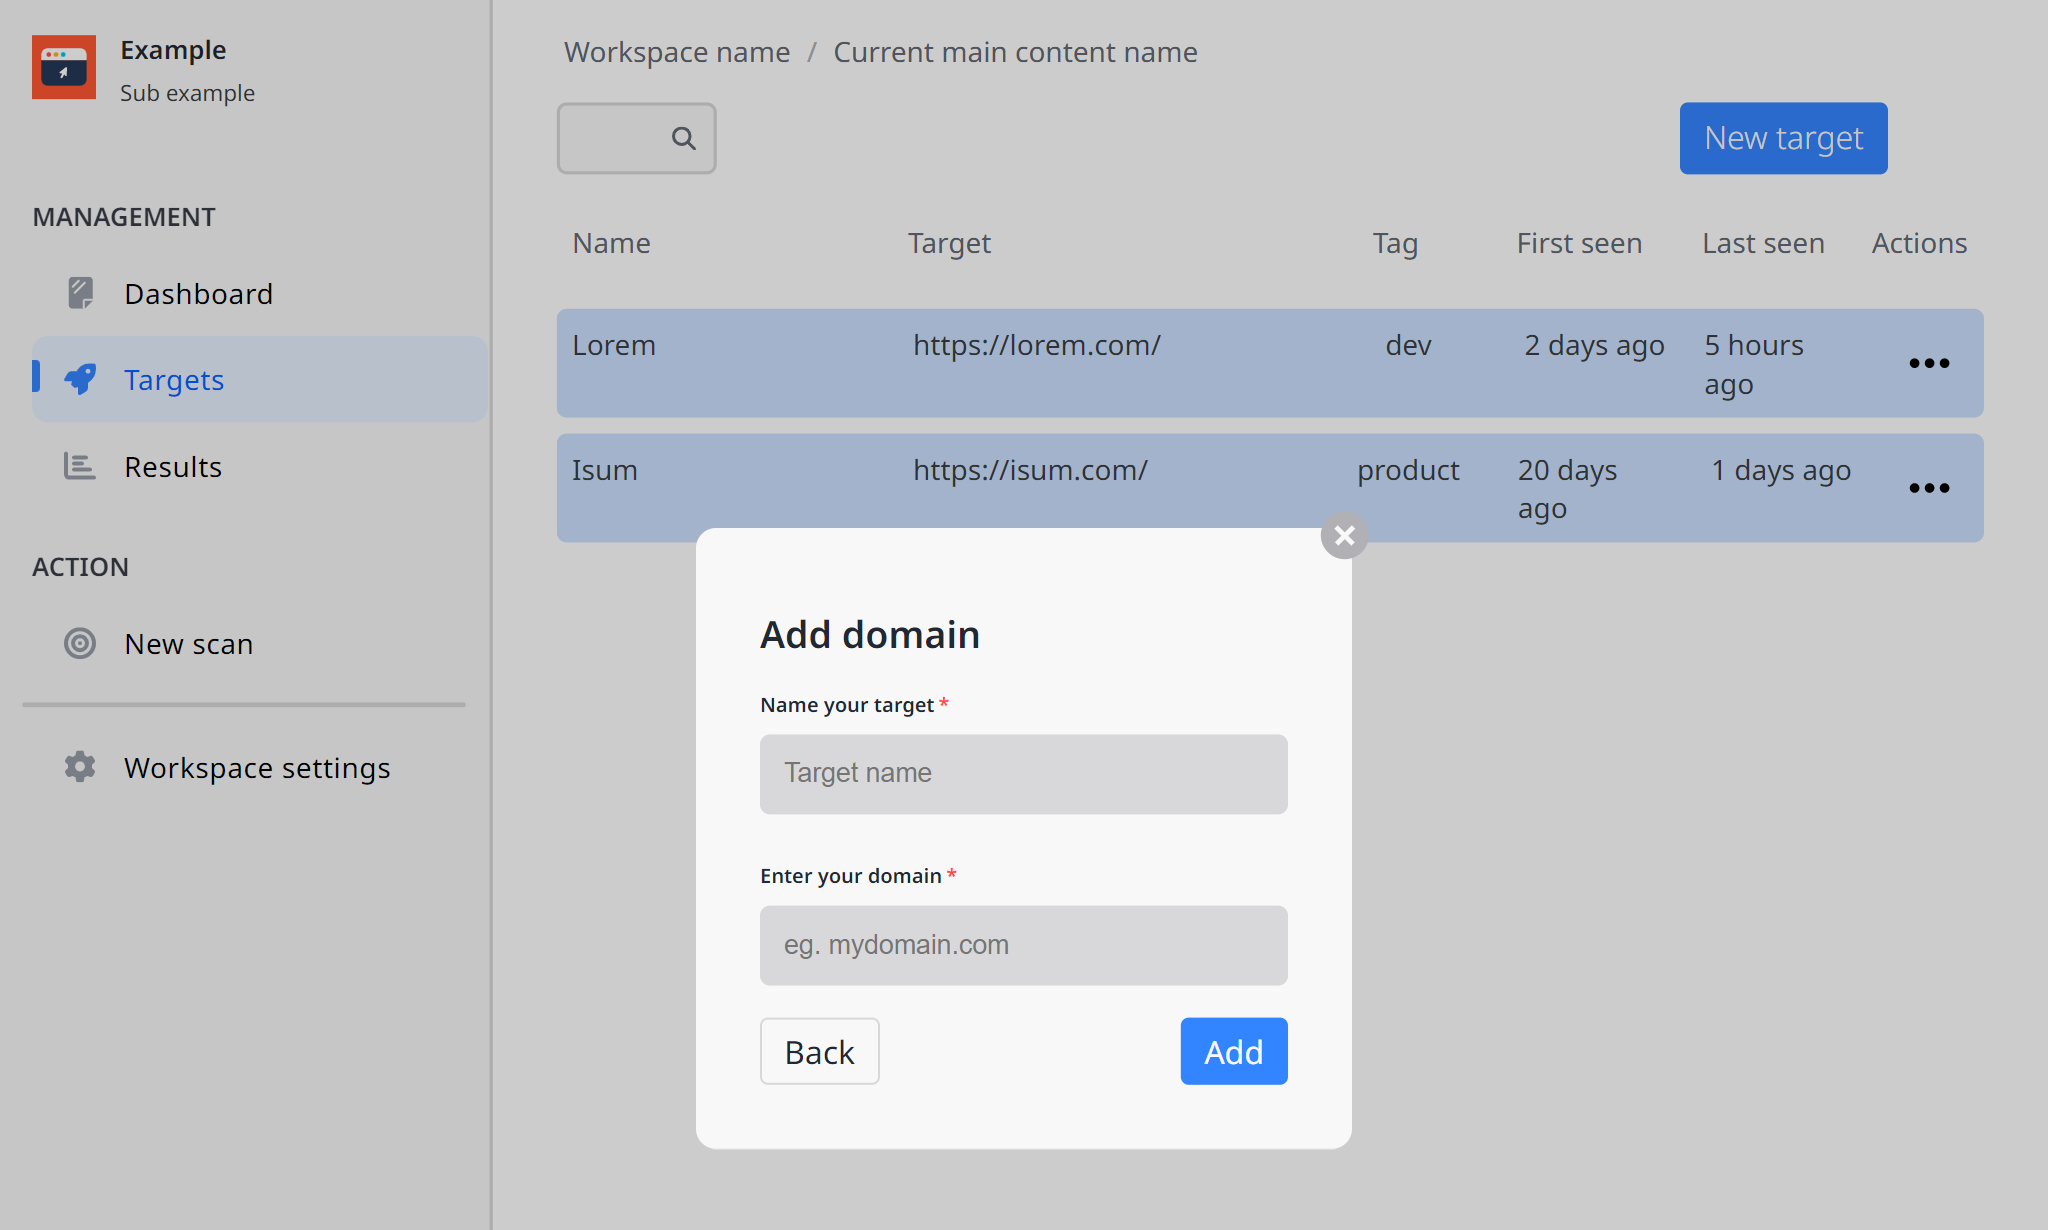
\includegraphics[width=\textwidth]{images/prototype/prototype_22112022/dashboard_target_add target_add domain.png}
    \caption{Màn hình trang thêm mới mục tiêu của ứng dụng 2}
\end{figure}

\begin{figure}[H]
    \centering
    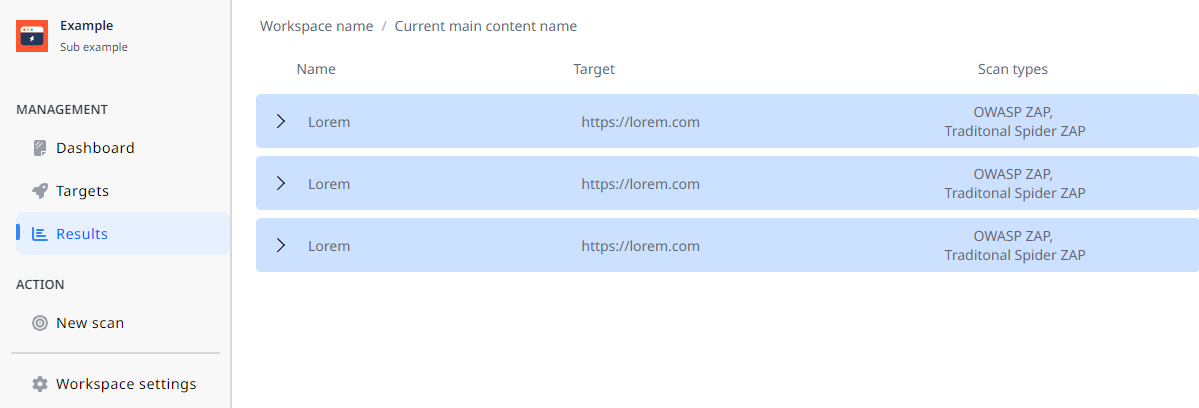
\includegraphics[width=\textwidth]{images/prototype/prototype_25102022/dashboard_result.png}
    \caption{Màn hình trang quản lý thông tin phiên quét của ứng dụng}
\end{figure}

\begin{figure}[H]
    \centering
    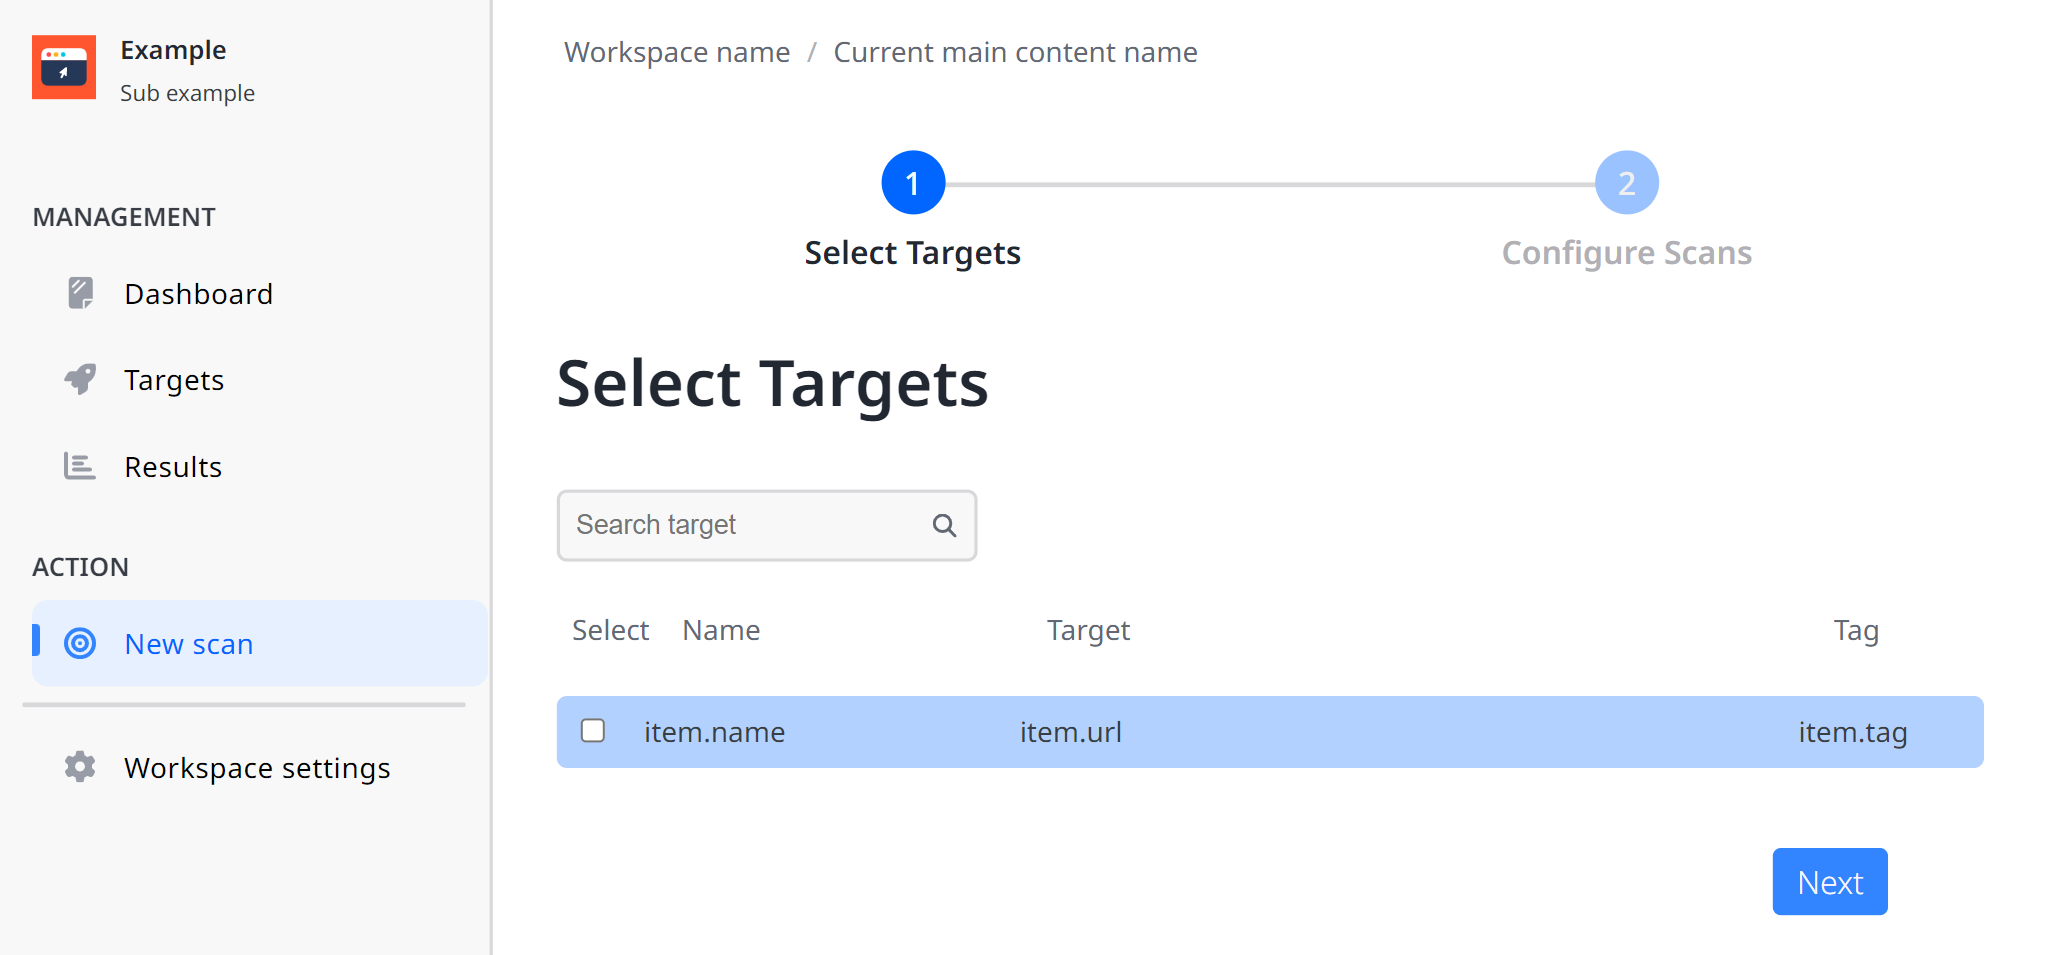
\includegraphics[width=\textwidth]{images/prototype/prototype_22112022/dashboad_new scan_select target.png}
    \caption{Màn hình trang tạo phiên quét của ứng dụng}
\end{figure}

\begin{figure}[H]
    \centering
    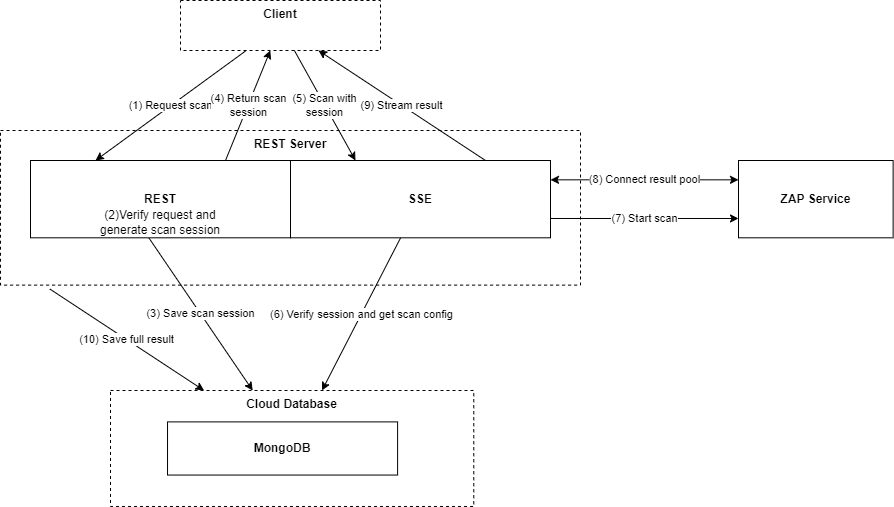
\includegraphics[width=\textwidth]{images/diagram/diagram_04112023/Scan Process.png}
    \caption{Hình thiết kế dự kiến cho quá trình thực hiện phiên quét của hệ thống}
\end{figure}

\myparagraph{Kiến trúc triển khai}

\begin{figure}[H]
    \centering
    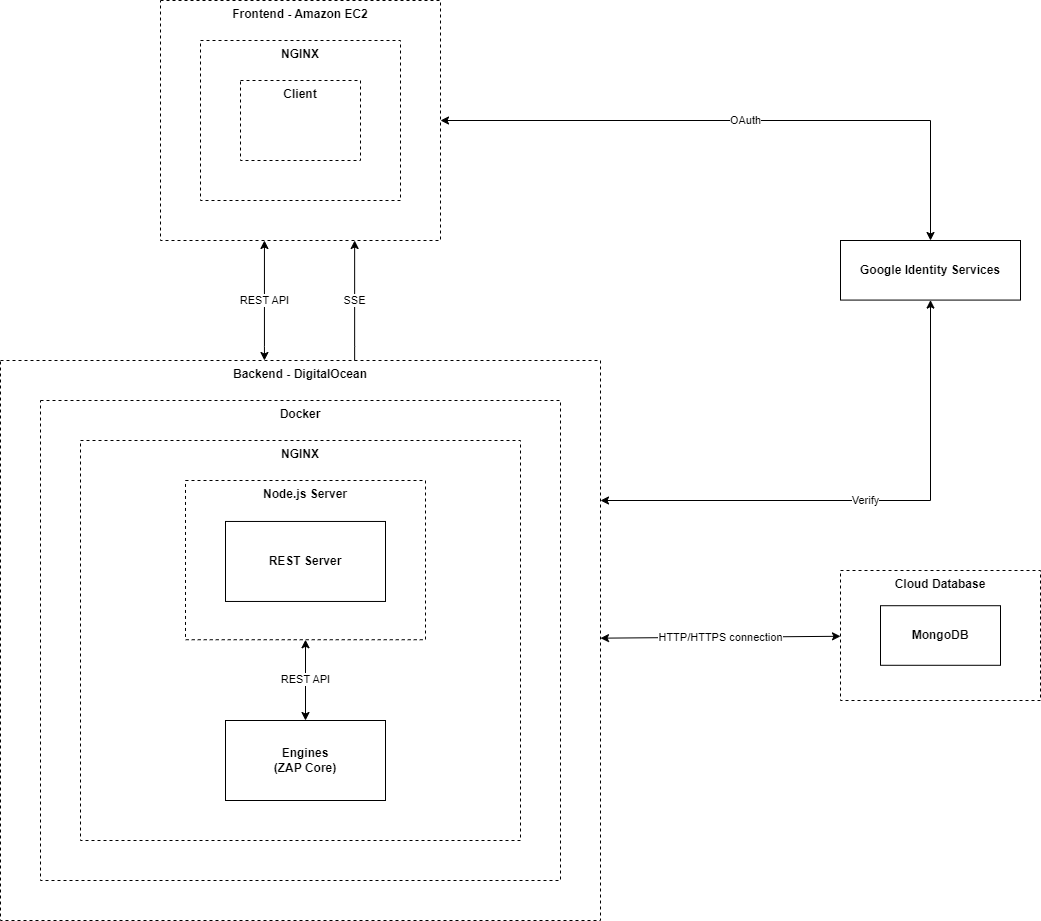
\includegraphics[width=\textwidth]{images/diagram/diagram_04112023/ZAPOP Architecture.png}
    \caption{Hình thiết kế dự kiến cho kiến trúc triển khai của hệ thống}
\end{figure}

\myparagraph{Mô hình dữ liệu}

\begin{figure}[H]
    \centering
    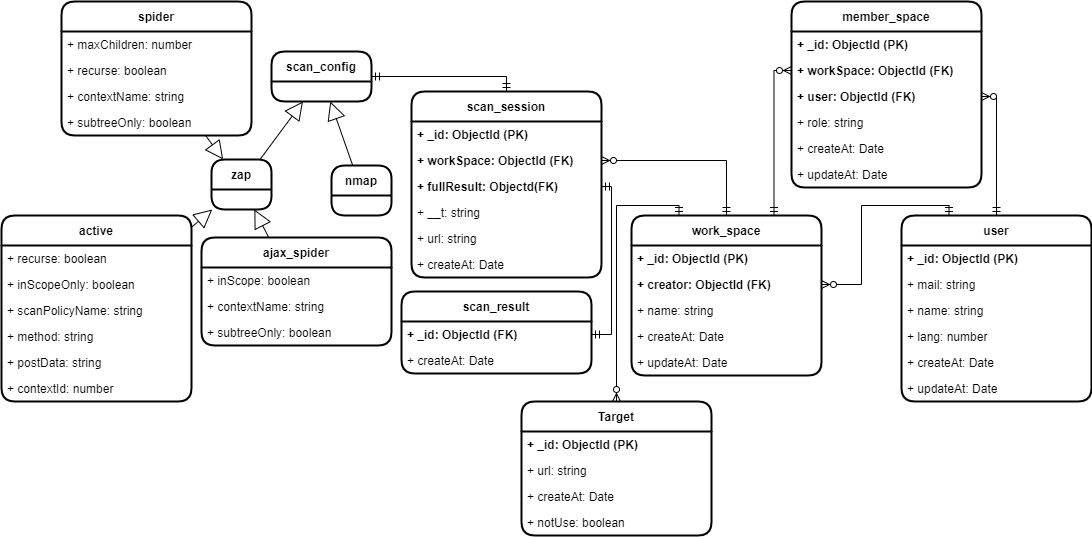
\includegraphics[width=\textwidth]{images/diagram/diagram_25102022/Database Diagram.png}
    \caption{Hình thiết kế dự kiến cho mô hình dữ liệu của hệ thống}
\end{figure}

\textbf{Bảng so sánh các tính năng cơ bản của các hệ thống}

\begin{tabularx}{\textwidth}{|>{\hsize=.25\hsize\centering\let\newline
    \\\arraybackslash}X|>{\hsize=.15\hsize\centering\let\newline
    \\\arraybackslash}X|>{\hsize=.15\hsize\centering\let\newline
    \\\arraybackslash}X|>{\hsize=.15\hsize\centering\let\newline
    \\\arraybackslash}X|>{\hsize=.15\hsize\centering\let\newline
    \\\arraybackslash}X|}
    \hline
    \textbf{Tính năng}
     & \textbf{\applicationname}
     & \textbf{Stack Hawk}
     & \textbf{Detectify}
     & \textbf{Hosted Scan}
    \\
    \hline
    Quét với ZAP
     &
    \checkmark
     &
    \checkmark
     &
    \checkmark
     &
    \checkmark
    \\
    \hline
    \caption{Bảng so sánh các tính năng cơ bản của các hệ thống}
\end{tabularx}

\textbf{Bảng ưu điểm và khuyết điểm của các hệ thống}

\begin{tabularx}{\textwidth}{|>{\hsize=0.2\hsize\centering\let\newline
    \\\arraybackslash}X|>{\hsize=0.4\hsize\raggedright\let\newline
    \\\arraybackslash}X|>{\hsize=0.4\hsize\raggedright\let\newline
    \\\arraybackslash}X|}
    \hline
    \thead{Hệ thống}
     &
    \thead{Ưu điểm}
     &
    \thead{Khuyết điểm}
    \\
    \hline
    Stack Hawk
     &
    - Tự động quét trên mỗi PR hoặc trong CI/CD.
    \newlinecontenttable
    - Quản lý thông tin kết quả quét, giao diện tường minh, dễ sử dụng.
    \newlinecontenttable
    - Đề xuất liên kết chứa thông tin sửa lỗi tìm được.
    \newlinecontenttable
    - Tích hợp được với những công cụ quản lý khác có sử dụng CI/CD như: Jira Sotfware, Gitlab, Github Action, Azure Pinelines, Jenkins, Travis CI,\dots
    \newlinecontenttable
    - Tài liệu hướng dẫn đầy đủ, chi tiết.
     &
    - Cần cấu hình pineline (.yml, .yaml).
    \newlinecontenttable
    - Cần Docker image đã build xây dựng sẵn.
    \newlinecontenttable
    - Kích hoạt quét bằng command line ở máy local. Cấu hình kích hoạt quét gồm nhiều bước.
    \newlinecontenttable
    - Dùng thử một lần mỗi ngày.
    \\
    \hline
    Hosted Scan
     &
    - Hỗ trợ các loại quét khác như Nmap, OpenVas, SSL/TLS.
    \newlinecontenttable
    - Hẹn thời gian đặt lịch quét.
    \newlinecontenttable
    - Đề xuất liên kết chứa thông tin sửa lỗi tìm được.
    \newlinecontenttable
    - Thông tin scan đầy đủ. Giao diện đơn giản.
     &
    - Kết quả scan dường như là dữ liệu gốc, không được xử lý.
    \newlinecontenttable
    - Dùng thử 10 lần mỗi tháng.
    \\
    \hline
    Detectify
     &
    - Tích hợp với các công cụ khác như: Slack, Jira, Zapier,…
    \newlinecontenttable
    - Đề xuất liên kết chứa thông tin sửa lỗi tìm được.
     &
    - Chi phí sử dụng cao.
    \newlinecontenttable
    - Cần phải cấu hình bên trong ứng dụng và triển khai để xác nhận chính chủ phức tạp, có thể không thành công.
    \newlinecontenttable
    - Không theo dõi được quá trình, tiến độ quét.
    \\
    \hline
    \caption{Bảng ưu điểm và khuyết điểm của các hệ thống}
\end{tabularx}

\myparagraph{Đánh giá}
\tab \tab - Các hệ thống tương tự đang có trên thị trường khá đa dạng.
Tuy nhiên, đa phần, mỗi hệ thống đều chỉ tập trung vào một chức năng nhất định trong các loại kiểm thử bảo mật.
Các hệ thống còn lại có chức năng bao quát như \applicationname có các tính năng mở rộng kèm theo thì yêu cầu nhiều bước cấu hình từ đầu gây ra việc khó sử dụng khi người dùng cần thực hiện công việc đơn giản nhanh chóng.
Tiếp đó là các hệ thống không trực quan trong quá trình quét hoặc là hiển thị kết quả quét chưa được xử lý hợp lý.
\par

- Qua so sánh, đánh giá hệ thống của nhóm với các hệ thống tương tự. 
Các thành viên nhóm đã đưa ra thống nhất tổng quan về hệ thống \applicationname Thực hiện đúng các kế
hoạch đề ra theo các mục 2.2 Mục tiêu đề tài và 2.3 Phạm vi của đề tài.

\paragraph{Danh sách các công nghệ, công cụ sử dụng}
\begin{itemize}
    \item Jira Software: một công cụ trong bộ công cụ của ứng dụng quản lý Jira, sử dụng mô hình Kanban để thiết kế và triển khai đồ án.
    \item Confluence: một công cụ trong bộ công cụ của ứng dụng quản lý Jira, dùng để quản lý tài liệu.
    \item GitHub: dịch vụ lưu trữ và kiễm soát phiên bản mã nguồn sử dụng Git.
    \item GitHub Pages: dịch vụ được tạo bởi GitHub, cho phép xuất bản trang web hoặc ứng dụng website bằng cách lưu trữ mã nguồn trong GitHub.
    \item Node.js: môi trường thực thi mã JavaScript bên ngoài trình duyệt.
    \item MongoDB: cơ sở dữ liệu dạng NoSQL.
    \item MongoDB Atlas: cloud database của MongoDB.
    \item Mongoose: a Node.js-based Object Data Modeling (ODM) library for MongoDB.
    \item OWASP Zed Attack Proxy (ZAP): ứng dụng mã nguồn mở dùng để quét lỗ hổng bảo mật của ứng dụng website.
    \item Express.js: framework dành cho backend Node.js của ứng dụng website.
    \item Server-Send Events - SSEs: một loại thiết hệ thống được xây dựng trên kết nối HTTP. Duy trì kết nối giữa frontend và backend tuy nhiên chỉ có backend được phép gửi dữ liệu lên.
    \item Docker: nền tảng để cung cấp các bước triển khai ứng dụng dễ dàng hơn bằng cách sử dụng các containers.
    \item DigitalOcean: một nhà cung cấp dịch vụ cloud và Cơ sở hạ tầng Dịch vụ (Infrastructure as a Service - IaaS).
    \item Amazon - Elastic Compute Cloud - EC2: một dịch vụ AWS cung cấp môi trường cloud computing cho phép người dùng thuê và sử dụng các máy ảo (Virtual machine - VM) trên cloud.
    \item NGINX: một web server cũng có thể được dùng để revese proxy, load balancer, mail proxy.
    \item ReactJS: thư viện JavaScript dùng để xây dựng giao diện website cho người dùng.
    \item Redux: thư viện JavaScript dùng để quản lý và xử lý trạng thái ứng dụng.
    \item Google Identity Services API: dùng để thực hiện định danh bằng Google.
    \item Visual Studio Code: trình biên tập mã được phát triển bởi Microsoft.
\end{itemize}